In diesem Grundlagenkapitel werden Erfolgschancen für Unternehmen aufgelistet, die Cloud-Dienste in ihre Geschäftsprozesse integrieren. Mit Cloud-Diensten sind die Dienste eines beliebigen Cloud-Anbieters im Allgemeinen gemeint und nicht ausschließlich AWS-Dienste. 
Es wird ebenfalls erklärt warum Kostenoptimierung und -überwachung relevant für Unternehmen sind.
\\\\
Folgende Ergebnisse könnten durch die Einführung von Überwachungs- und Optimierungsmaßnahmen erreicht werden:
\begin{itemize}
      \item
            Die Möglichkeit, die Kosten verschiedener Projekte, die über dieselbe Infrastruktur laufen, zu trennen.
            Auf diese Weise kann zwischen Projekten, die mehr, und Projekten, die weniger Kosten verursachen unterschieden werden.%Davor Kunden und nicht Projekte
      \item
            Eine beachtliche Erhöhung der finanziellen Rentabilität im Unternehmen.%[ZITAT].
      \item
            Eine geringere Ungewissheit bei der Umsetzung von cloudbasierten Systemen.
      \item
            Mehr Kontrolle über die Gesamtkosten des Betriebs, den sogenannten \textit{TCO}.\footnote{Vgl. TCO: Total Cost if Ownership}\footnote{Vgl. Ubuntu, delivered by Canonical: A business guide to hybrid/multi-cloud, S.2.\cite{CAN01}}

\end{itemize}
%Basandose en "Vor- und Nachteile der Nutzung von Cloud-Diensten (mit mobilen Endgeräten) in Organisationen und deren Einfluss auf die Nachhaltigkeit"
% Debería aclarar los aspectos principales de mi BA
% En mi caso: 

%1-Cuales son los miedos, razones y oportunidades para las empresas en la NUBE?

%\subsection{Risiken und Oportunitäten der Cloud...}\label{subsec_UabsGrund2}
%Vor- und Nachteile / ?

\subsection{Cloud Economics}\label{subsec_UabsGrund3}
%Was bietet die Cloud den Unternehmen?
%Economics of Cloud Computing
%https://d1.awsstatic.com/whitepapers/introduction-to-aws-cloud-economics-final.pdf
%[Date last review: 25.11 Isa]
\begin{flushleft}
%\textit{On-Demand Prinzip} kann zum Beispiel die Rechenkapazität je nach Bedarf angepasst werden 
\textit{Cloud Economics} befasst sich mit den Kosten und den Vorteilen von Cloud Computing und die dahinterstehenden wirtschaftlichen Grundsätzen. Anhand des \textit{Pay-as-you-go-Modell(PAYG)} können zum Beispiel nur die Cloud-Dienste in Anspruch genommen werden, die in dem Moment für das Unternehmen verbraucht werden. Damit entfällt die Notwendigkeit hohe Investitionen in Hardware zu tätigen, wie bei On-Premise-Systemen, wo Hardware im Voraus für den künftigen Bedarf.\footnote{Vgl. Anders Lisdorf, 2021, Cloud Computing Basics: a Non.-Technical Introduction, S.23\cite{CCB}} Durch den Verzicht auf Hardware entfallen die Kosten für Reparatur und Wartung. Cloud-Anbieter übernehmen viele Verwaltungsaufgaben. Laut Larry Carvalho und Matthew Marden führe dies zu einer Abnahme der nötigen Fachkräften.\footnote{Vgl. Larry Carvalho and Matthew Marden, 2015, Quantifying the Business Value of Amazon Web Services, S.1\cite{IDC01}} So ist die die Nutzung von Cloud-Diensten in unabhängiger Weise möglich; in Selbstbedienung und mit der Freiheit Dienste ohne Einschränkungen zu gebrauchen. Das bedeutet jedoch gleichzeitig, dass die Nutzerin oder der Nutzer von Cloud-Diensten Verantwortung für die anfallenden Kosten übernehmen.
\end{flushleft}
%[Grafik der Kosten On-Premise/Demand?]

\subsubsection{Skalierbarkeit}
Skalierbarkeit bezieht sich in dieser Arbeit auf die Möglichkeit, die Kapazität von Cloud-Diensten zu skalieren. Um die Leistung der IT-Infrastruktur aufrecht zu halten, ist es zum Beispiel möglich, das Serversystem so zu konfigurieren, dass es auf wechselnde Lastanforderungen reagiert.
%bietet  ist es möglich die Rechenkapazität hoch- und runterzuskalieren.
%Vertikal und Horizontal
%
%DOPPELT?Mit Auto Scaling wird sichergestellt, dass die Rechenkapazität in Zeiträumen von hoher Nachfrage automatisch hochskaliert.[AUCH RUNTER?]
% davor:  Anzahl der Amazon Server-Instanzen ABER ANZAHL VON SERVERN != Rechenkap.
% und damit Kosten minimieren.
Auf diese Weise kann Zeit mit der Verwaltung von IT-Infrastruktur eingespart werden, welche dann genutzt werden kann, um sich auf die wesentlichen Geschäftsaktivitäten zu konzentrieren.
\footnote{Mark Wilkins, 2021, AWS Certified Solutions Architect - Associate (SAA-C02), S.29.\cite{AWS1}}
%\parencite[][Seite 29]{AWS1} 
%\footnote{Vgl. [p.~29]\cite{AWS1}[]}
%OPTION 2: 
%Auf diese Weise wird Zeit mit der Verwaltung von IT-Ressourcen gespart und es kann sich auf die wesentlichen Geschäftsaktivitäten konzentrieren.
% Davor: 
%Auf diese Weise kann weniger Zeit mit der Verwaltung von IT-Ressourcen verbracht werden und sich mehr auf wesentliche Geschäftsaktivitäten konzentriert werden\footnote{Vgl. {\cite{AWS1}}, Seite 29}.
%\\\\
Dies war der Fall bei \textit{Walgreens} im Jahre 2020 in den Vereinigte Staaten.
Sie haben unter anderem 750 virtuelle Maschinen und \textit{SAP HANA} auf \textit{Azure Instanzen} migriert.
Diesbezüglich kommentierte Dan Regalado:
\begin{quote}
      By getting out of the business of managing datacenters, WBA[Walgreens Boots Alliance] can spend less time worrying about managing IT resources and more time focusing on what it’s really good at—delivering great healthcare and retail experiences to its customers. Azure also gives WBA an opportunity to better utilize the capabilities of its SAP implementation. “One of the key reasons for moving to Azure was so that we could take advantage of the scalability that SAP HANA is capable of,” explains Regalado. “Instead of using extremely big SAP HANA Large Instances, we can start using smaller VMs[virtuelle Maschinen] and then scale out.\footnote{Microsoft, 2020, Customer Story-Walgreens Boots Alliance delivers superior customer service with SAP solutions on Azure, o.S. \cite{AZU01}}
\end{quote}
So erklärte Dan Regalado, dass \textit{Walgreens} mit dem Einsatz von kleinen Instanzen und Auto-Scaling eine Serverinfrastruktur erreicht hat, die sich dem Bedarf an Rechenkapazität anpasst. 

\subsubsection{Flexibilität}% und Agilität}
Hiermit ist die Möglichkeit Cloud-Dienste in Auftrag zu geben und kündigen zu können gemeint, wenn sie nicht mehr benötigt werden. Das unter den mit dem Cloud-Anbieter vereinbarten Bedingungen.
Für Cloud-Dienste gibt es im Allgemeinen eine Vielzahl von Optionen, von denen einige Beispiele unten aufgeführt werden:
\begin{itemize}
\item
    Verschiedene Betriebssysteme, ohne oder mit Lizenzierung.
\item
    Die meistverbreiteten Programmiersprachen, unter anderem \textit{Java, C++, Go, JavaScript und Python}.{\cite{AMZ03}}
\item
    Hosting für statische Webseiten und Webanwendungen{\cite{AMZ04}}.
\item
    Populäre relationale und nicht relationale Datenbanken{\cite{AMZ10}}.           
\item
    Vielfältige Hardware-Konfigurationen.

\end{itemize}
\begin{flushleft}
Durch die Vielzahl der verfügbaren Diensten ist es möglich, Prototypen und Experimente in kurzer Zeit durchzuführen.\footnote{Vgl. IDC, 2015, Business Value of AWS S.7\cite{IDC01}} Softwareprojekte können schnell auf den Markt gebracht werden. Je nach ihrem Erfolg ist es möglich, sinnvolle Entscheidungen zu treffen. Wenn ein Projekt, aus welchen Gründen auch immer, kurzfristig eingestellt werden muss, könnten alle damit verbundenen Kosten ausfallen. Denn im Gegensatz zu On-Premise-Infrastrukturen gibt es keine Bindung an kostspielige Hardware.
      %Wenn die Neuentwicklung nicht erfolgreich war, müssen keine weitere Kosten anfallen.
      %Da die verwendete Dienste vollständig stillgelegt werden können.
\end{flushleft}

\subsubsection{Selbstbedienung}
Mit geringem Aufwand ist es möglich, Cloud-Dienste eigenständig einzurichten. Dies hat den Vorteil, dass keine weiteren Personen wie externe Spezialisten oder die Vertriebsabteilung des Cloud-Anbieters  benötigt werden.\footnote{Vgl. Anders Lisdorf, 2021, Cloud Computing Basics: a Non.-Technical Introduction, S.28\cite{CCB}}
Andererseits besteht die Gefahr, dass hohe ungewollte Kosten entstehen, wenn jemand versehentlich oder in unverantwortlicher Weise Dienstleistungen in Anspruch nimmt.    
%[TODO: ADD USE CASE WHERE THIS HAPPEND]
%LinkedIn Learning, the woman said something like that?
%BRINGT DIESE UNTERKAP. ETWAS ZUR ARBEIT BEI?

\subsubsection{Keine Vorabkosten}
%https://aws.amazon.com/de/ec2/pricing/
Das Pay-as-you-go-Modell(PAYG) wird von einer Reihe von Cloud-Anbietern angeboten.\footnote{Vgl.  Die aktuellen Marktführer im Bereich der \textit{Cloud-Computing} weltweit sind AWS, Google, Telekom und Microsoft (Vgl. Synergy Reseach Group 2019, o.S.\cite{STA6}} Dies erfordert keine Vorauszahlungen für die Nutzung von vielen Cloud-Diensten. Wenn nur für die monatlich verbrauchten Diensten bezahlt wird, verringert sich die Anfangsinvestition in die IT-Infrastruktur oder fällt ganz weg. Dies ist besonders für kleine Unternehmen interessant, die nicht über die finanziellen Mittel verfügen, um in eine IT-Infrastruktur zu investieren. Es besteht jedoch die Möglichkeit, bestimmte Beträge für die zu konsumierende Dienste im Voraus zu bezahlen. Im Unterkapitel \ref{sssec:Vorauszahlung} wird eine Berechnung der Einsparungen durch die teilweise oder vollständige Vorauszahlung der Kosten für die Nutzung von Serverinstanzen gezeigt.  

%\subsubsection{Verfügbarkeit?} t.ly/bV1z
\subsubsection{Technische Fachkompetenz}
Bei einem Einsatz von Cloud-Diensten ist zu bedenken, dass weitere Investitionen wie technische Schulungen für das Personal erforderlich werden. \textit{TÜV Rheinland} bietet zum Beispiel Kurse zur Ausbildung von Cloud Architekten an. Die Kurse dauern drei Tage und kosten 2.136,05 € pro Teilnehmer. Maßnahmen wie die genannten Kurse wirken einem der Hauptprobleme entgegen, mit denen Unternehmen bei der Migration in die Cloud konfrontiert werden. In der von Accenture im Jahr 2020 durchgeführten Umfrage gaben 38\% der Befragten an, dass fehlende Kompetenzen im Unternehmen im Bezug auf die Cloud ein Hindernis für eine Cloud-Migration ist.\footnote{Vgl. Accenture Dienstleistungen GmbH. Hohe Erwartungen an die Cloud: Hürden
meistern, Mehrwert maximieren, S.11\cite{ACC1}}
%[KOSTEN EINER IT-INFRA = SERVER+Rack]
% QUE PORTENTAJE DE LA INVERSION REPRESENTA LA INFRAESTRUCTURA DE IT EN UNA START UP Y EN UNA CORPORACION? RAZONES USAR LA NUBE(Statista)?

\subsection{Amazon Cloud-Dienste}%Sarah 6.12
Im Folgenden liegt der Fokus auf \textit{AWS-Diensten}. Einer der am häufigsten genutzten AWS-Dienste ist \textit{Amazon Elastic Computing Instances EC2}, mit dem virtuelle Maschinen erstellt werden können.\footnote{Vgl.  Kimberly Mlitz, 2021, Cloud infrastructure services vendor market share worldwide from 4th quarter 2017 to 3rd quarter 2021, o.S.\cite{STA4}} Ein weiterer wichtiger AWS-Dienst ist \textit{Amazon Simple Storage Service (S3)}, der zum Speichern von Objekten verwendet wird.\footnote{Vgl. Objekte sind in AWS die Grundeinheit in welchen Dateien in den Amazon S3-Speichereinheiten gespeichert werden. Neben den Objekten werden Metadaten, wie das Datum der Objekterstellung und das Datum der letzten Aktualisierung gespeichert.} Amazon Elastic Computing Instances EC2 werden im Folgenden in dieser Arbeit als \textit{EC2-Instanzen} und Amazon Simple Storage Service als \textit{Amazon S3} oder \textit{Amazon S3-Speichereinheiten} bezeichnet.
\\\\
Wie Lynn Langit, eine erfahrene Cloud-Architektin, feststellte, könne bis zu 80\% der AWS-Rechnung aus Gebühren für EC2-Instanzen bestehen.\footnote{Vgl. Lynn Langit, 2021, LinkedIn Learning: AWS Controlling Cost. Minute 0:20-0:45\cite{LINK2}} Laut des \textit{AWS Solutions Architekten} Daniel Peña Silva ist Amazon S3 einer der am häufigsten genutzten AWS-Dienste.\footnote{Vgl. Daniel Peña Silva, 2021, LinkedIn: Listado de todos los Servicios de AWS.\cite{LINK1}} Deshalb fokussiert sich diese Arbeit auf die Überwachungs- und Optimierungsmaßnahmen, hauptsächlich für EC2-Instanzen und Amazon S3.  %\subsubsection*{Amazon Elastic Computing Instances EC2}
%, Sektion 2 Control Costs by Service, Video AWS service type Minute 00:30}.%\subsubsection*{Amazon Simple Storage Service S3} Warum S3 t.ly/iWn3
%S3 ist der Speicherdienst für Objekte bei AWS. 
%der Rangliste vieler Informatikwebseiten und 
%BESSER: S3 WIRD IN BÜCHER WIE t.ly/IJc1 GENANNT? THIS IS A SPANISH CITAT!
\\\\
Wie aus der \autoref{fig:moreCloudStorageThanLocal} hervorgeht ist, werden darüber hinaus seit 2020 weltweit mehr Daten in Serverfarmen als auf lokalen Geräten gespeichert.\footnote{Vgl. Statista: 2020 überholt die Cloud lokale Speichermedien.\cite{STA1}} Dies bietet Vorteile im Bezug auf die Geschwindigkeit der Arbeitsabläufe, birgt aber auch Risiken wie Datendiebstahl. Das Thema Datendiebstahl wird in dieser Arbeit nicht behandelt.%; da es den Rahmen der Untersuchung sprengen würde.
\begin{figure}[h!]
      \centering
      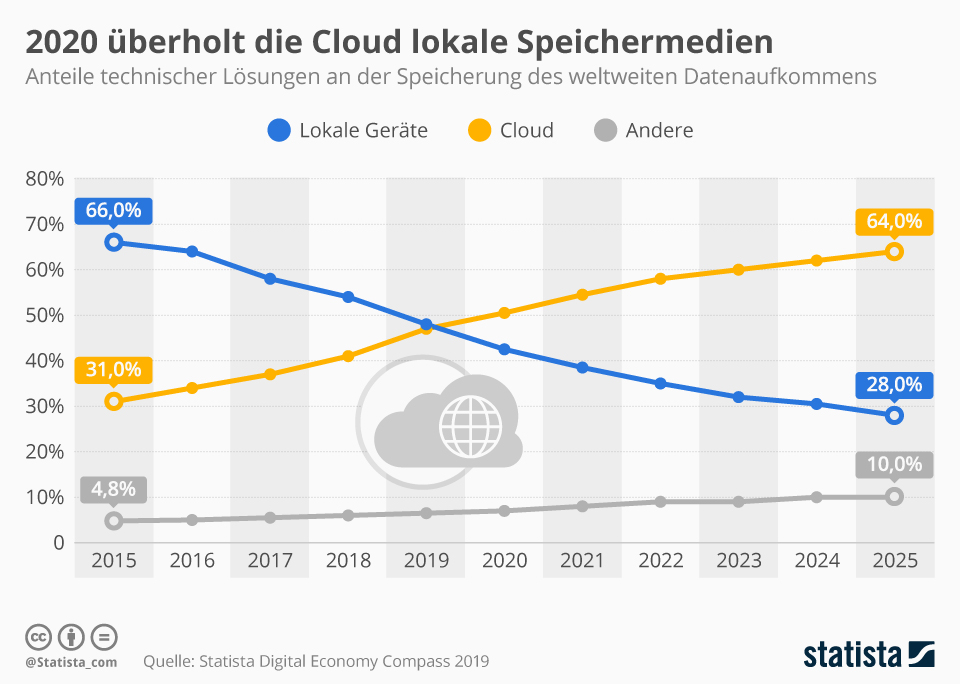
\includegraphics[scale=0.4]{sources/moreCloudStorageThanLocal}
      \caption[2020 überholt die Cloud lokale Speichermedien]{}\label{fig:moreCloudStorageThanLocal}
      2020 überholt die Cloud lokale Speichermedien, Statista, 2019 {\cite{STA1}}
\end{figure}
\\\\
\\\\
\\\\
Dieses grundlegende Kapitel hat einige potenzielle Vorteile der Nutzung von Cloud-Diensten für Unternehmen aufgezeigt. Darüber hinaus geht der Trend in den letzten Jahren zur Nutzung von Cloud-basierten Diensten. Das nächste Kapitel befasst sich mit den Zahlungsmodellen für EC2-Instanzen und den Überlegungen, die bei der Wahl dieser Modelle in verschiedenen Szenarien zu berücksichtigen sind.
\newpage

\begin{comment}
Advantages of Cloud Technology
As the technology has matured over the last decade, companies are moving to the
cloud to lower costs, reduce complexity, and increase flexibility. The cloud
provides scalable and powerful compute solutions, low-cost, reliable storage, and addition, cloud technologies can be used to deploy solutions quickly and cost effectively around the world and on any device.
When you decouple from the data center, you’ll be able to:
x Decrease your TCO: Eliminate many of the costs related to building and
maintaining a data center or colocation deployment. Pay for only the
resources you consume.

x Reduce complexity: Reduce the need to manage infrastructure,
investigate licensing issues, or divert resources.
x Adjust capacity on the fly: Add or reduce resources, depending on
seasonal business needs, using infrastructure that is secure, reliable, and
broadly accessible.
x Reduce time to market: Design and develop new IT projects faster.
x Deploy quickly, even worldwide: Deploy applications across multiple
geographic areas.
x Increase efficiencies: Use automation to reduce or eliminate IT
management activities that waste time and resources.
x Innovate more: Spin up a new server and try out an idea. Each project
moves through the funnel more quickly because the cloud makes it faster
(and cheaper) to deploy, test, and launch new products and services.
x Spend your resources strategically: Switch to a DevOps model to free
your IT staff from operations and maintenance that can be handled by the
cloud services provider.
x Enhance security: Spend less time conducting security reviews on
infrastructure. Mature cloud providers have teams of people who focus on
security, offering best practices to ensure you’re compliant, no matter what
your industry.
\end{comment}

%\subsection{Was ist EC2? To Review}\label{subsec_UabsGrund4}
%Man kann HW und SW auswählen


% Amazon video Cloud Eco.: https://www.youtube.com/watch?v=kUNBx1MTwxw
% short explaniation https://www.youtube.com/watch?v=RI9RTbXEjLc
%3- Hard and Soft Savings https://youtu.be/Q5wSvUVPyYY?t=316
% Suche ein Buch, mit info darüber!

